\documentclass[%
 reprint,
 amsmath,amssymb,
 aps,
]{revtex4-2}
\usepackage{balance}
\usepackage[%
    margin=10mm,% ако не си принтира 10мм не изглежда грозно, а може да събереш повече текст
    % showframe=true,%
    ]{geometry}
\usepackage[T1,T2A]{fontenc}
\usepackage[utf8]{inputenc}
\usepackage[main=bulgarian, english]{babel}
\usepackage{float}
\AtBeginDocument{\selectlanguage{bulgarian}}
\newcommand{\degree}{^{\circ}}
\usepackage{amsmath}
\usepackage{graphics}
\usepackage{graphicx}
\graphicspath{{.}}
\newcommand{\abs}[1]{\lvert#1\rvert}
\let\phi\varphi
\usepackage{booktabs} % от тук се използва само \midrule може и без него 
\usepackage{dcolumn}
\newcolumntype{d}[1]{D{.}{.}{#1}}
\usepackage[unicode=true,pdfusetitle]{hyperref}
\usepackage[]{siunitx}

\usepackage[compact]{titlesec}


\begin{document}
\setlength{\abovedisplayskip}{3pt}
\setlength{\belowdisplayskip}{3pt}    

\title{Термодвойка}
\author{Васил Николов}
\date{08.03.2022}
\maketitle
%%\balance

\section{Цел на упражнението}

Да се определи експериментално коефициентът на вътрешно триене на въздух $\eta$, и да се пресметне дължината на средния свободен пробег на молекули във въздуха. 

\section{Експериментална установка}

В основата на експеримента е тънка капилярка, през която преминава въздух. Тя е с дължина $l=13.35 \ \si{mm^2}$ и диаметър $d = 0.5 \ \si{mm}$. От едната си страна капилярката е свързана чрез маркуч към изсушител на въздух, а от другата - към запечатана колба с вода. Колбата има кранче на дъното си, и когато то се отвори и нивото на водата започне да спада, през капилярката се засмуква въздух. Изсушителят на въздух е голяма епруветка, пълна със соли, които поглъщат водните пари, които преминават около тях. В голямата епруветка се поставя стъклена тръбичка, единият край на която е свързан с маркуча към капилярката, а другият е заровен под повърхността на солта. Така когато въздух влиза в капилярката той задължително е преминал покрай солите, и голяма част от водната пара в него е премахната. От двете страни на капилярката е свързан воден манометър, който ще мери разликата в наляганията от двете й страни. Тази разлика ще се използва във формулата за пресмятане на коефициентът на вътрешно триене. На фигура \ref{fig:1} е представена схема на установката. 

\begin{figure}[H] 
    \centering
    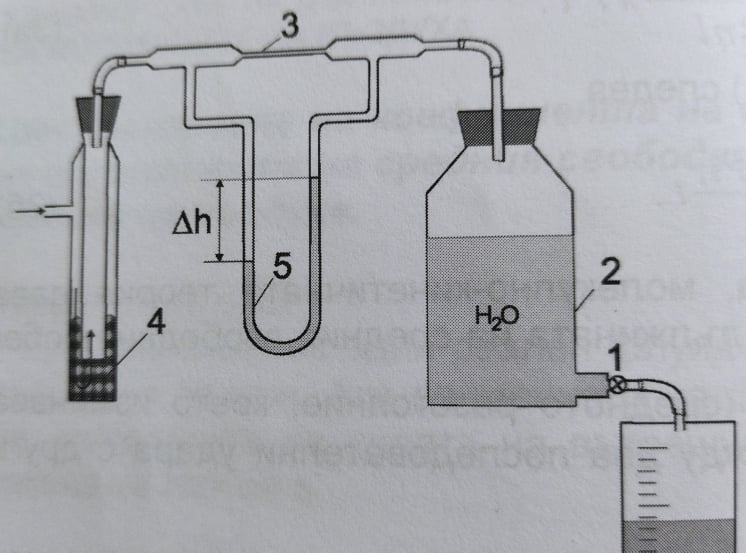
\includegraphics[width=0.9\columnwidth, keepaspectratio=true]{scheme_1.jpg}
    \caption{Схема на установката}\label{fig:1} 
\end{figure}

\section{Теоретична обосновка}

За ламинарен поток на флуид през тръба е валиден законът на Нютон: 

\begin{equation*}
    Q = \frac{\Delta P}{8\eta l}\pi r^4
\end{equation*}

Ако приемем разликата в наляганията в началото и края на тръбата за постоянни с времето то можем да пресметнем обемът въздух, преминал за някакъв интервал от време $\Delta t$ по формулата

\begin{equation*}
    V = Q\Delta t = \frac{\Delta P}{8\eta l}\pi r^4 \Delta t
\end{equation*}

Но тъй като разликата в наляганията в началото и краят на капилярката е много по-малък от атмосферното налягане, то той е равен на обемът изтекла течност. Тогава ако премерим за колко време изтича даден обем вода, в нашия случай $V = 500 \ \si{ml}$, то можем да пресметнем коефициентът на вътрешно триене на въздуха $\eta$ по формулата 

\begin{equation*}
    \eta = \frac{\pi r^4 \Delta P}{8Vl}t \label{eq:1} \tag{1}
\end{equation*}

Знаейки стойността на коефициентът на вътрешно съпротивление на възудха можем да сметнем стойността му по следната формулата

\begin{gather*}
    \bar{\lambda} = \frac{3\eta}{\rho \bar{u}} = \frac{3\eta}{p} \sqrt[]{\frac{\pi RT}{8\mu}} \label{eq:2} \tag{2} \\ 
    \bar{u} = \sqrt[]{\frac{8kT}{\pi m}} = \sqrt[]{\frac{8RT}{\pi \mu}} 
\end{gather*}

Тук $\bar{u}$ е средната скорост на молекулите $p$ е въздушното налягане и $T$ е стайната температура. 

\section{Експериментални данни и резултати}

Експериментът се състои в това да се пусне да изтича вода от колбата, и едновременно с това се пуска таймер, мери се разликата в наляганията от двете страни на манометъра по време на изтичането, и се спира таймерът точно когато е изтекъл $V = 500 \ \si{ml}$ обем вода. За по-голяма точност експериментът се повтаря 10 пъти при различна скорост на изтичане на водата. В таблицата са дадени измерените стойности на разликата в наляганията за 10те измервания

\begin{table}[H]
    \centering
    \begin{tabular}{@{}llr@{}} \toprule
    t, s  & P, cm & P, cm \\
    \midrule
    110.3 & 4.1        & 4.2        \\
    105.9 & 3.5        & 3.7        \\
    37.6  & 13.8       & 14.2       \\
    57.4  & 7.6        & 7.4        \\
    127.4 & 2.7        & 2.5        \\
    114.7 & 3.2        & 3.2        \\
    34.9  & 13.8       & 13.6       \\
    63.7  & 6.4        & 6.2        \\
    108.5 & 3.4        & 3.4        \\
    \bottomrule
    \end{tabular}% 
\end{table}

За всяка една от стойностите е пресметнато числото на Рейнолдс 

\begin{equation*}
    Re = \frac{\rho Q}{\eta \pi r} 
\end{equation*}

При всяко едно измерване числото на Рейнолдс е по-малко от критичната стойност $Re_{crit} = 1200$, така че няма нужда да премахваме експериментални данни. Тогава пресмятаме средната стойност на коефициентът на вътрешно триене на въздуха $\overline{\eta} = 1.50*10^{-5} \ \si{Pa.s} \pm 5\%$

С така намереният коефициент на вътрешно триене можем по формула \eqref{eq:2} да пресметнем стойност за средният свободен пробег $\bar{\lambda} = 86 \ \si[]{nm}$.

\end{document}